% !TeX root = ../libro.tex
% !TeX encoding = utf8
\setchapterpreamble[c][0.75\linewidth]{%
	\sffamily
	Volterra empezó a trabajar en las ecuaciones integrales en 1884, pero el nombre de \textit{ecuación integral} se lo dio Bois-Reymond en 1888. Sin embargo, el término \textit{ecuación integral de Volterra} se utilizó por primera vez en 1908 por el matemático rumano Traian Lalesco.
	\par\bigskip
}
\chapter{Métodos de resolución de ecuaciones integrales de Volterra de segunda clase}

\section{Introducción}
Para recopilar información sobre los métodos, hemos tomado como referencia \cite{WazWaz}.

El diseño de métodos numéricos para ecuaciones integrales en general, y en particular de Volterra, es un campo de investigación vigente actualmente.
Existen una gran variedad de métodos numéricos y analíticos, tales como el método de aproximaciones sucesivas, la transformada de Laplace, colocación con splines, Runge-Kutta, y otros muchos que han sido utilizados para manejar las ecuaciones integrales de Volterra.

A parte de estudiar algunos de estos métodos tradicionales, veremos otros métodos algo más recientes tales como:
\begin{itemize}
	\item Método de descomposición de Adomian (ADM)
	\item Método de descomposición modificado (mADM)
	\item Método de iteración variacional (VIM)
\end{itemize}
Nos vamos a centrar principalmente en cómo se aplican estos métodos con un objetivo principal, encontrar una solución $u(x)$ para la ecuación integral de Volterra de segunda clase.\\Daremos una visión general de esta amplia familia de métodos de resolución, sin entrar en detalles como la convergencia o el error.

Para diferenciar mejor en qué se basan cada uno de los métodos, vamos a distinguir entre los métodos que utilizan series, los métodos iterativos, y otros métodos especiales que no se engloban en los anteriores.
\section{Métodos basados en series}
\subsection{Método de descomposición de Adomian (ADM)}
Fue desarrollado por George Adomian en \cite{Adomian1} y \cite{Adomian12} y está muy bien abordado en muchas referencias. Se ha investigado mucho sobre este método para poder aplicarlo a una amplia clase de ecuaciones diferenciales ordinarias, en derivadas parciales, y también en ecuaciones integrales (véase \cite{Atkinson}).

Consiste en expresar una función $u(x)$ como una serie de descomposición definida por
\begin{equation}\label{eq:sum_adomian}
	u(x) = \sum_{n=0}^{\infty} u_n(x),
\end{equation} 
convergente en algún sentido, donde las componentes $u_n(x), n \geqslant 0$, tienen que ser determinadas de una forma recursiva. El método se ocupa de encontrar las componentes $u_0, u_1, u_2, ...,$ individualmente. Como ya veremos más adelante, se pueden hallar estas componentes de una forma sencilla a través de una relación de recurrencia que normalmente implica integrales simples que pueden ser fácilmente evaluadas.

Para establecer la relación de recurrencia, sustituimos~\eqref{eq:sum_adomian} en la ecuación integral de Volterra~\eqref{eq:volterra} para obtener 
\begin{equation}
	\sum_{n=0}^{\infty} u_n(x) = f(x) + \int_{0}^{x} K(x,t)(\sum_{n=0}^{\infty} u_n(t))dt,
\end{equation}
o equivalentemente
\begin{equation}
	u_0(x) + u_1(x) + u_2(x) + \cdots = f(x) + \int_{0}^{x} K(x,t)[u_0(t) + u_1(t) + \cdots]dt.
\end{equation}
La primera componente $u_0(x)$ se identifica con todos los términos que no están incluidos dentro de la integral. Por lo tanto, las componentes $u_j(x), j \geqslant 1$, de la función desconocida $u(x),$ están completamente determinadas a través de la siguiente relación de recurrencia:
\begin{align}
	u_0(x) &= f(x),      &   \\
	u_{n+1}(x) &=  \int_{0}^{x} K(x,t)u_n(t)dt, \qquad n \geqslant 0,         & 
\end{align}
que es equivalente a 
\begin{align}\label{eq:recurrencia1}
	u_0(x)&=f(x),          &  u_1(x) &= \int_{0}^{x} K(x,t)u_0(t)dt,      \\
	u_2(x)&= \int_{0}^{x} K(x,t)u_1(t)dt,   &  u_3(x)&= \int_{0}^{x} K(x,t)u_2(t)dt, 
\end{align}
y análogamente para las demás componentes. Como podemos ver en~\eqref{eq:recurrencia1}, las componentes $u_0(x), u_1(x), u_2(x), u_3(x),..., u_n(x)$ están completamente determinadas. Como resultado, la solución $u(x)$ de la ecuación integral de Volterra~\eqref{eq:volterra} en forma de serie se obtiene fácilmente utilizando~\eqref{eq:sum_adomian}.

\begin{observacion}
Hemos visto cómo el método de descomposición ha convertido una ecuación integral en una determinación de componentes calculables. Muchos investigadores formalizaron que si existe una solución exacta para el problema, entonces la serie obtenida converge muy rápidamente a esa solución (véase \cite{WazWaz}).

Sin embargo, para problemas concretos donde no se puede obtener una solución, generalmente se utiliza un número truncado de términos con fines numéricos. Podemos observar que cuantos más componentes usemos, mayor precisión obtendremos, ya que la sucesión formada por los componentes converge a la solución.
\end{observacion}

\begin{ejemplo}
	Resolveremos la siguiente ecuación integral de Volterra utilizando el ADM:
	\begin{equation}
		u(x) = 1 - \int_{0}^{x} u(t)dt.
	\end{equation}
	En este caso, $f(x) = 1, \lambda = -1, K(x,t) = 1.$ Se asume que la solución $u(x)$ tiene una forma en serie como la dada en~\eqref{eq:sum_adomian}. Sustituyendo la serie en ambos lados de nuestra ecuación, obtenemos:
	\begin{equation}
		\sum_{n=0}^{\infty} u_n(x) = 1 - \int_{0}^{x} \sum_{n=0}^{\infty} u_n(t)dt.
	\end{equation}
	La primera componente corresponde con todos los términos que no están incluidos dentro de la integral, por tanto, obtenemos la siguiente recurrencia:
	\begin{align}
		u_0(x) &= 1,      &   \\
		u_{k+1}(x) &= - \int_{0}^{x} u_k(t)dt, \qquad k \geqslant 0,         & 
	\end{align}
	por tanto, tenemos:
	\begin{align}
		u_0(x) &= 1,      &   \\
		u_{1}(x) &= - \int_{0}^{x} u_0(t)dt = -\int_{0}^{x} 1dt = -x,    &  \\
		u_{2}(x) &= - \int_{0}^{x} u_1(t)dt = -\int_{0}^{x} (-t)dt = \dfrac{1}{2!}x^2,    &  \\
		u_{3}(x) &= - \int_{0}^{x} u_2(t)dt = -\int_{0}^{x} \dfrac{1}{2!}t^2dt = \dfrac{1}{3!}x^3.    & 
	\end{align}	
	Así, obtenemos la solución en serie:
	\begin{equation}
		u(x) = 1 - x + \dfrac{1}{2!}x^2 - \dfrac{1}{3!}x^3 + \cdots,
	\end{equation}
	que converge a la solución:
	\begin{equation}
		u(x) = e^{-x}.
	\end{equation}
\end{ejemplo}

\subsection{Método de descomposición modificado (mADM)}
Wazwaz presenta una modificación importante del ADM en sus libros \cite{WazWaz1} y \cite{WazWaz2}. Este método facilitará el proceso de cálculo y acelerará la convergencia de la solución en series. Se aplicará, siempre que se pueda, a cualquier ecuación integral y diferencial de cualquier orden.
\begin{observacion}
	Este método se basa principalmente en dividir la función $f(x)$ en dos partes, por tanto no se puede usar si la función $f(x)$ está formada por un sólo término.
\end{observacion}
El método de descomposición modificado introduce una pequeña variación a la relación de recurrencia que vimos en el ADM, y esto nos llevará a la determinación de las componentes de $u(x)$ de una forma más fácil y rápida.

En muchos casos, la función $f(x)$ se puede escribir como una suma de dos funciones parciales, llamadas $f_1(x)$ y $f_2(x)$:
\begin{equation}
	f(x) = f_1(x) + f_2(x).
\end{equation}
Gracias a esto, se introducirá un cambio importante a la hora de formar la relación de recurrencia en el método de Adomian. Para minimizar el tamaño de los cálculos, identificamos la primera componente $u_0(x)$ como una de las partes de $f(x)$, que será $f_1(x)$ o $f_2(x)$. La otra parte se puede añadir a la componente $u_1(x)$ junto a los demás términos. En resumen, obtenemos la siguiente relación de recurrencia:
\begin{align}
	u_0(x) &= f_1(x),      &   \\
	u_{1}(x) &= f_2(x) + \lambda \int_{0}^{x} K(x,t)u_0(t)dt,    &  \\
	u_{k+1}(x) &= \lambda \int_{0}^{x} K(x,t)u_k(t)dt, \qquad k \geqslant 1.    &
\end{align}	
\begin{observacion}
	Esto muestra que la diferencia entre la relación de recurrencia estándar y la modificada se basa únicamente en la formación de las dos primeras componentes $u_0(x)$ y $u_1(x)$. Las demás componentes se mantienen igual.
\end{observacion}
Aunque esta variación en las dos primeras componentes es pequeña, WazWaz afirma en su libro \cite{WazWaz} que juega un papel muy importante en acelerar la convergencia de la solución y en minimizar la cantidad de trabajo computacional. Además, varios trabajos de investigación han confirmado que reducir el número de componentes en $f_1(x)$ afecta a todas las componentes, no sólo a $u_1(x)$.

A continuación vamos a ver dos observaciones importantes a cerca de este método:
\begin{observacion}
	Si elegimos correctamente las funciones $f_1(x)$ y $f_2(x)$, podremos obtener la solución exacta $u(x)$ utilizando muy pocas iteraciones, incluso algunas veces evaluando sólo dos componentes. De hecho, el éxito de esta modificación depende de hacer una buena elección de las funciones $f_1(x)$ y $f_2(x)$, y la forma de obtenerlas adecuadamente es a través de prueba y error, ya que no se ha encontrado todavía una regla para facilitar esta elección.
\end{observacion}

\begin{observacion}
	Si $f(x)$ está formada sólo por un término, el método recae en el método de descomposición de Adomian.
\end{observacion}

Podemos utilizar este método para las ecuaciones integrales tanto de Volterra como de Fredholm, lineales en nuestro caso. Vamos a ver un ejemplo utilizando este método, y compararemos la solución con la del método de Adomian para 5 iteraciones y así podremos apreciar la diferencia en cuanto a la rapidez de convergencia:

\begin{ejemplo}
	Resolver la ecuación integral de Volterra:
	\begin{equation}
		u(x) = 1 -x-\dfrac{1}{2}x^2 - \int_{0}^{x}(t-x) u(t)dt.
	\end{equation}
	La función $f(x)$ está compuesta por 3 términos, que están fuera de la integral, y vamos a dividirlos en dos partes de la siguiente forma:
	\begin{align}
		f_1(x) &= 1 -x,      &   \\
		f_2(x) &=-\dfrac{1}{2}x^2.    &
	\end{align}
	Y ahora utilizamos la fórmula de recurrencia modificada, obteniendo:
	\begin{align}
		u_0(x) &=  1 -x,      &   \\
		u_{1}(x) &=-\dfrac{1}{2}x^2 - \int_{0}^{x}(t-x) u_0(t)dt = 0,    &  \\
		u_{k+1}(x) &= - \int_{0}^{x}(t-x) u_k(t)dt, \qquad k \geqslant 1.    &
	\end{align}
	En la quinta iteración obtenemos:
	\begin{equation}
		u_5(x)=-\dfrac{x^9}{120960}.
	\end{equation}
	Hemos obtenido la solución exacta para esta ecuación gracias a \textit{Maxima}:
	\begin{equation}
		u(x) = 1 - \sinh(x).
	\end{equation}
	Ahora vamos a mostrar gráficamente en la \autoref{fig:adomian1} la solución que nos da el método de Adomian y el modificado para 5 iteraciones comparándolos con la solución exacta:
	\begin{figure}[h!]
		\centering
		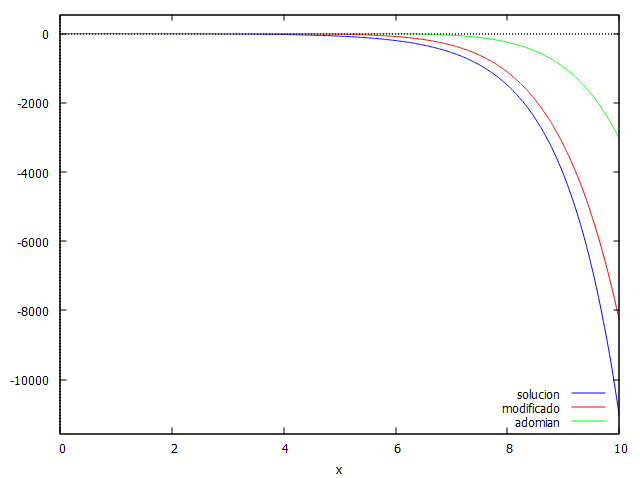
\includegraphics[width=0.8\textwidth]{ejemplo_adomian}
		\caption{Comparación de la solución para 5 iteraciones con el método de Adomian y el método modificado}
		\label{fig:adomian1}
	\end{figure}
	\begin{observacion}
		Podemos ver como efectivamente la convergencia en el método modificado es mucho más rápida que en el método de Adomian ya que con sólo 5 iteraciones ya se aproxima mucho mejor a la solución.
\end{observacion}
\end{ejemplo}

\subsection{Método de la solución en series}
\begin{definicion}
	Una función real $u(x)$ se llama \textit{analítica} si existe derivada de cualquier orden de forma que la serie de Taylor en cualquier punto $b$ de su dominio
	\begin{equation}
		u(x) = \sum_{k=0}^{\infty}\dfrac{f^{(k)}(b)}{k!}(x-b)^k,
	\end{equation}
	converge a $f(x)$ en un entorno de $b$.
\end{definicion}
Por simplicidad, escribiremos la forma genérica de la serie de Taylor en $x = 0$ como
\begin{equation}\label{eq:serie1}
	u(x) = \sum_{n=0}^{\infty}a_nx^n.
\end{equation}
\begin{observacion}
	Si $f$ es analítica en todo punto de un intervalo $I$, entonces, la propia definición nos garantiza que $f \in \mathcal{C}^\infty(I)$. Sin embargo, el recíproco no es cierto, como prueba el siguiente ejemplo bien conocido (véase en \cite{ejemploanalitica}):
	\begin{ejemplo}
		Sea la función
		\begin{equation}
			f(x) = \left\lbrace\begin{array}{c} e^{-1/x^2} \qquad x > 0 \\ 0 \qquad \qquad x \leqslant 0 \end{array}\right.
		\end{equation}
		Esta función es $\mathcal{C}^\infty(\R)$, ya que todas sus derivadas existen y son continuas en cualquier punto. Sin embargo, no es analítica en $x = 0$. La serie de Taylor alrededor de $x=0$ se reduce a una serie de potencias de ceros. Por lo tanto, no se puede representar como una serie de potencias convergente en un entorno de $x=0$.
	\end{ejemplo}
\end{observacion}
Vamos a presentar un método muy útil, que se basa principalmente en la serie de Taylor para funciones analíticas, y resolverá ecuaciones integrales de Volterra. Podemos apreciar que guarda cierta similitud con Adomian, ya que de igual forma expresamos $u$ como la suma de cierta serie.

Asumimos que la solución $u(x)$ de la ecuación integral de Volterra
\begin{equation}
	u(x) = f(x) + \int_0^x K(x,t)u(t)dt,
\end{equation}
es analítica, es decir, posee una solución en forma de serie de Taylor, donde los coeficientes $a_n$ se determinarán de forma recursiva. Sustituimos~\eqref{eq:serie1} en ambos lados y obtenemos
\begin{equation}\label{eq:serie2}
	\sum_{n=0}^{\infty}a_nx^n = T(f(x)) + \int_{0}^{x}K(x,t)(\sum_{n=0}^{\infty}a_nt^n)dt,
\end{equation}
o por simplicidad usamos
\begin{equation}
	a_o + a_1x + a_2x^2 + \cdots = T(f(x)) + \int_{0}^{x}K(x,t) (a_0+a_1t+a_2t^2+\cdots)dt,
\end{equation}
donde $T(f(x))$ es la serie de Taylor para $f(x)$. La ecuación integral se convertirá en una integral tradicional donde en vez de integrar la función desconocida $u(x)$, se integrarán términos de la forma $t^n,n\geqslant0$. Al estar en búsqueda de una solución en series, si la función $f(x)$ incluye funciones elementales, deberemos incluir sus desarrollos en forma de Taylor.

Primero integramos la parte derecha de la integral en~\eqref{eq:serie2} y tomamos los coeficientes de las potencias de $x$. Después igualamos los coeficientes de ambos lados para obtener una relación de recurrencia con $a_j, j\geqslant0$. Resolver la recurrencia nos llevará a determinar completamente los coeficientes $a_j, j\geqslant0$.

Ahora la solución en series se sigue inmediatamente de sustituir estos coeficientes. La solución exacta se obtendrá si existe, y si no, la serie obtenida se podrá utilizar con objetivos numéricos. En este caso, a más términos evaluemos, mayor precisión obtendremos.

Veamos un ejemplo para dejar claro este método:
\begin{ejemplo}
	Vamos a resolver la ecuación integral de Volterra
	\begin{equation}
		u(x) = 1 - x \sin x + \int_{0}^{x} tu(t)dt.
	\end{equation}
	Sustituyendo la serie en ambos lados y utilizando la expansión en serie de Taylor para el seno obtenemos:
	\begin{equation}
		a_0 + a_1x + a_2x^2 + a_3x^3 + a_4x^4 +\cdots = 1 - x(x-\dfrac{x^3}{3!} + \cdots) + \int_{0}^{x}t(a_0+a_1t+a_2t^2+\cdots)dt.
	\end{equation}
	Integrando el lado derecho y quedándonos con los coeficientes encontramos
	\begin{equation}
		a_0 + a_1x + a_2x^2 + a_3x^3 + a_4x^4 + \cdots = 1+(\dfrac{1}{2}a_0-1)x^2+\dfrac{1}{3}a_1x^3+(\dfrac{1}{6}+\dfrac{1}{4}a_2)x^4+\cdots
	\end{equation}
	Igualando los coeficientes de las potencias de $x$,
	\begin{align}
		a_0&=1,          &  a_1&=0,      \\
		a_2&=\dfrac{1}{2}a_0-1,   &  a_3&=\dfrac{1}{3}a_1 = 0, \\
		a_4&=\dfrac{1}{6}+\dfrac{1}{4}a_2 = \dfrac{1}{4!},
	\end{align}
	y para $n\geqslant0$,
	\begin{equation}
		a_{2n+1} = 0, \qquad a_{2n} = \dfrac{(-1)^n}{(2n)!}, \qquad n \geqslant 0.
	\end{equation}
	La solución en forma de serie viene dada por
	\begin{equation}
		u(x) = 1 - \dfrac{1}{2!}x^2 + \dfrac{1}{4!}x^4-\dfrac{1}{6!}x^6+\cdots
	\end{equation}
	que nos da la solución exacta
	\begin{equation}
		u(x) = \cos x.
	\end{equation}
	En la \autoref{fig:sol_suma} mostramos la comparación de la suma parcial $v(x) = 1 - \dfrac{1}{2!}x^2 + \dfrac{1}{4!}x^4-\dfrac{1}{6!}x^6+\dfrac{1}{8!}x^8$ con la solución exacta $u(x)$, se aprecia que la aproximación es bastante buena.
	\begin{figure}[h!]
		\centering
		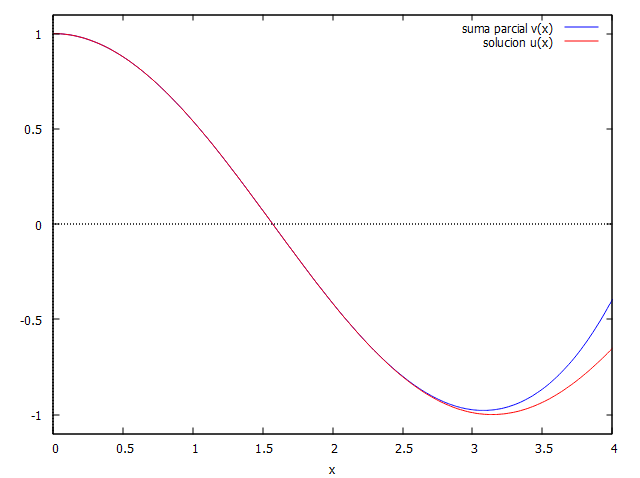
\includegraphics[width=0.8\textwidth]{suma_parcial_sol}
		\caption{Comparación de la solución exacta con la suma parcial $v(x)$}
		\label{fig:sol_suma}
	\end{figure}
\end{ejemplo}

\section{Métodos iterativos}

\subsection{Método de iteración variacional (VIM)}
Este método ha sido desarrollado por Ji-Huan He en sus libros \cite{VIM1} y \cite{VIM2}, y ha demostrado ser eficaz y seguro para estudios numéricos y analíticos. El método proporciona aproximaciones sucesivas que convergen rápidamente a la solución exacta en forma de serie, siempre que exista. Sin embargo, en el caso de que no se pueda obtener la solución exacta, la serie resultante se puede utilizar para fines numéricos. Asimismo, una de las ventajas que tiene este método es que puede abordar problemas tanto lineales como no lineales de la misma forma sin necesidad de añadir más restricciones. Vamos a presentar los pasos principales del método:

Consideramos la ecuación diferencial:
\begin{equation}\label{eq:miv1}
	Lu + Nu = g(t),
\end{equation}
donde \textit{L y N} son operadores lineales y no lineales respectivamente , y $g(t)$ es el término no homogéneo.

El método de iteración variacional presenta un funcional de corrección para la ecuación~\eqref{eq:miv1} de la forma:
\begin{equation}\label{eq:miv2}
	u_{n+1}(x) = u_n(x) + \int_{0}^{x} \lambda(\xi)(Lu_n(\xi) + N\tilde{u}_n(\xi) - g(\xi))d\xi,
\end{equation}
donde $\lambda$ es un multiplicador de Lagrange general.
\begin{observacion}
	Nótese que en este método, $\lambda$ puede ser una constante o una función, y $\tilde{u}_n$ es un valor restringido, por tanto se comporta como una constante, luego $ \tilde{u}'_n = 0$.
\end{observacion}
Para un uso completo de este método, deberíamos seguir dos pasos:
\begin{enumerate}
	\item Determinar el multiplicador de Lagrange $\lambda(\xi)$ que será identificado de forma óptima.
	\item Una vez determinado $\lambda$, sustituimos el resultado en~\eqref{eq:miv2} donde se deberían omitir las restricciones.
\end{enumerate}
Derivando en~\eqref{eq:miv2} con respecto a la variable independiente $u_n$, obtenemos
\begin{equation}
	\dfrac{d u_{n+1}}{d u_n} = 1 + \dfrac{d}{d u_n}(\int_{0}^{x} \lambda(\xi)(Lu_n(\xi)+N\tilde{u}_n(\xi)-g(\xi))d\xi),
\end{equation}
o equivalentemente si multiplicamos por $du_n$:
\begin{equation}\label{eq:miv3}
	d u_{n+1} = d u_n + (\int_{0}^{x} \lambda (\xi)(Lu_n(\xi))d\xi).
\end{equation}
Para determinar el multiplicador de Lagrange $\lambda(\xi)$ normalmente se utiliza la integración por partes. Por ejemplo, si tenemos $Lu_n(\xi) = u'_n(\xi)$ en~\eqref{eq:miv3}, entonces se convierte en
\begin{equation}
	d u_{n+1} = d u_n +(\int_{0}^{x} \lambda (\xi)(u'_n(\xi))d\xi).
\end{equation}
Integrando por partes obtenemos
\begin{equation}
	d u_{n+1} = d u_n + \lambda(\xi)u_n(\xi) - \int_{0}^{x} \lambda'(\xi) d u_n(\xi)d\xi.
\end{equation}
o equivalentemente
\begin{equation}
	d u_{n+1} = d u_n(\xi)(1 + \lambda |_{\xi = x}) - \int_{0}^{x} \lambda'd u_nd\xi.
\end{equation}
La condición final de $u_{n+1}$ requiere que $d u_{n+1} = 0$. Esto significa que la parte izquierda vale cero, y por tanto la parte derecha también debería valer cero, lo que nos lleva a las condiciones:
\begin{equation}
	1 + \lambda |_{\xi = x} = 0, \qquad \lambda'|_{\xi = x} = 0.
\end{equation}
Lo que al final nos da
\begin{equation}
	\lambda = -1.
\end{equation}
Una vez hemos determinado el multiplicador de Lagrange $\lambda(\xi)$, las sucesivas aproximaciones $u_{n+1}, n \geqslant 0$, de la solución $u(x)$ se obtendrán fácilmente al usar la función selectiva $u_0(x)$. Sin embargo, para una rápida convergencia, la función $u_0(x)$ se debe seleccionar utilizando las primeras condiciones como siguen:
\begin{align}
	u_0(x) &= u(0),  \shorteqnote{para la primera derivada $u'_n$}  &   \\
	u_0(x) &= u(0) + xu'(0),  \shorteqnote{para la segunda derivada $u''_n$}  &   \\
	u_0(x) &= u(0) + xu'(0) + \dfrac{1}{2!}x^2u''(0), \qquad \qquad \qquad \shorteqnote{para la tercera derivada $u'''_n$}
\end{align}
y así sucesivamente. Por tanto, tenemos la solución 
\begin{equation}
	u(x) = \lim_{n\rightarrow \infty} u_n(x).
\end{equation}
Es decir, el funcional de corrección nos dará varias aproximaciones, y por tanto, la solución exacta se obtiene como el límite de todas estas sucesivas aproximaciones.

La determinación del multiplicador de Lagrange juega un papel muy importante para llegar a la solución del problema. A continuación, mostramos un esquema correspondiente al multiplicador de Lagrange y su funcional de corrección para un caso general de orden n:
	\begin{align}
	u^{(n)} + f(u(\xi),u'(\xi&),...,u^{(n)}(\xi)) = 0, \lambda = (-1)^n\dfrac{1}{(n-1)!}(\xi - x)^{(n-1)},      &   \\
	u_{n+1} = u_n + (-1)^n & \int_{0}^{x} \dfrac{1}{(n-1)!}(\xi - x)^{(n-1)}[u'''_n + f(u_n,...,u^{(n)}_n)]d\xi,    &
\end{align}
para todo $n \geqslant 1$.

Para utilizar el método de iteración variacional y resolver ecuaciones integrales de Volterra, es necesario convertir la ecuación integral a un problema de valores iniciales equivalente o a una ecuación integro-diferencial.

Vamos a examinar el problema de valores iniciales obtenido utilizando el método de iteración variacional como veremos en el siguiente ejemplo:
\begin{ejemplo}
	Resolveremos la siguiente ecuación integral de Volterra usando el método de iteración variacional:
	\begin{equation}
		u(x) = 1 + \int_{0}^{x}u(t)dt.
	\end{equation}
	Usando el Teorema Fundamental del Cálculo para derivar ambos lados de la ecuación, obtenemos
	\begin{equation}\label{eq:miv4}
		u'(x) - u(x) = 0.
	\end{equation}
	Sustituyendo $x = 0$, tenemos la condición inicial $u(0) = 1.$ Ahora, utilizando el método de iteración variacional, el funcional de corrección para la ecuación~\eqref{eq:miv4} es
	\begin{equation}\label{eq:miv5}
		u_{n+1}(x) = u_n(x) + \int_{0}^{x} \lambda (\xi) (u'_n(\xi) - \tilde{u}_n(\xi))d\xi.
	\end{equation}
	Usando la fórmula del esquema visto anteriormente para el caso $n = 1$ llegamos a que 
	\begin{equation}
		\lambda = -1.
	\end{equation}
	Sustituyendo el valor del multiplicador de Lagrange $\lambda = -1$ en el funcional nos da la fórmula iterativa:
	\begin{equation}
		u_{n+1}(x) = u_n(x) - \int_{0}^{x} (u'_n(\xi) - u_n(\xi))d\xi.
	\end{equation}
	Como dijimos anteriormente, podemos usar la condición inicial $u_0(x) = u(0) = 1.$ Usando esta selección en~\eqref{eq:miv5} obtenemos las siguientes aproximaciones sucesivas:
	\begin{align}
		u_0(x) &= 1,      &   \\
		u_1(x) &= 1 - \int_{0}^{x} (u'_0(\xi) - u_0(\xi))d\xi = 1 + x,    & \\
		u_2(x) &= 1 + x - \int_{0}^{x} (u'_1(\xi) - u_1(\xi))d\xi = 1 + x + \dfrac{1}{2!}x^2,    & \\
		u_3(x) &= 1 + x + \dfrac{1}{2!}x^2 - \int_{0}^{x} (u'_2(\xi) - u_2(\xi))d\xi = 1 + x + \dfrac{1}{2!}x^2 + \dfrac{1}{3!}x^3,    &
	\end{align}
	y así sucesivamente. El VIM admite el uso de 
	\begin{align}
		u(x) &= \lim_{n \rightarrow \infty} u_n(x),      &   \\
		&= \lim_{n \rightarrow \infty} (1 + x + \dfrac{1}{2!}x^2 + \dfrac{1}{3!}x^3 + ... + \dfrac{1}{n!}x^n)
	\end{align}
	con lo que obtenemos la solución exacta
	\begin{equation}
		u(x) = e^x.
	\end{equation}
	En la \autoref{fig:sol_vim} mostramos la comparación de la suma parcial $v(x) = 1 + \dfrac{1}{2!}x^2 + \dfrac{1}{3!}x^3+\dfrac{1}{4!}x^4$ con la solución exacta $u(x)$, se aprecia que la aproximación es bastante buena.
	\begin{figure}[h!]
		\centering
		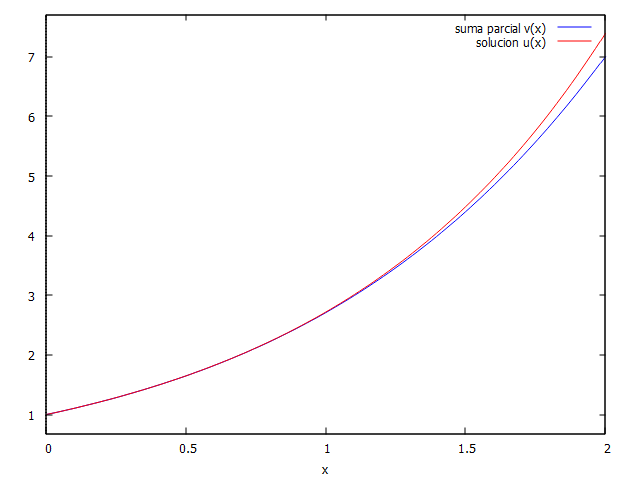
\includegraphics[width=0.8\textwidth]{grafica_vim}
		\caption{Comparación de la solución exacta con la suma parcial $v(x)$}
		\label{fig:sol_vim}
	\end{figure}
\end{ejemplo}

\subsection{Método de aproximaciones sucesivas}
El método de aproximaciones sucesivas, también conocido como el \textit{método de iteración de Picard}, nos proporciona un esquema que puede ser utilizado para resolver problemas de valores iniciales o ecuaciones integrales. Este método encuentra aproximaciones sucesivas que convergen a la solución a partir de una inicial, llamada la \textit{aproximación inicial}. Como veremos, la aproximación inicial puede ser cualquier función real que se utilizará en una relación recurrente para determinar las otras aproximaciones.

Dada la ecuación integral lineal de Volterra de segunda clase
\begin{equation}
	u(x) = f(x) +\int_{0}^{x} K(x,t)u(t)dt,
\end{equation}
donde $u(x)$ es la función desconocida a determinar, $K(x,t)$ es el núcleo, y $\lambda$ un parámetro. El método de las aproximaciones sucesivas introduce la siguiente relación de recurrencia
\begin{equation}\label{eq:wowo}
	u_n(x) = f(x) + \int_{0}^{x} K(x,t)u_{n-1}(t)dt, \qquad n \geqslant 1,
\end{equation}
donde la aproximación inicial $u_0(x)$ puede ser cualquier función real. Siempre empezamos con una suposición inicial para $u_0(x)$, normalmente se suele elegir $0$ ó $f(x)$.

La convergencia de $u_n(x)$ está justificada con el estudio del capítulo $2$, teniendo en cuenta que 
\begin{equation}
	u = \sum_{j=0}^{\infty}L^jf,
\end{equation}
siendo $L$ el operador lineal visto en~\eqref{ref_operador}, que 
\begin{equation}
	u_n = \sum_{j=0}^{n}L^jf,
\end{equation}
y que el papel de $f$ ($=u_0$) lo puede jugar cualquier otra función continua $g$, ya que se tendría:
\begin{align}
		u_0 &= g \\ u_1 &= f+Lg \\ \vdots \\ u_n &= (\sum_{j=0}^{n-1}L^jf)+L^ng.
\end{align}
donde $L^ng \rightarrow 0$. Es más, en el mencionado capítulo $2$ obtuvimos cotas del error para este método.
En la siguiente observación vamos a ver algunas diferencias entre los métodos iterativos que hemos visto.
\begin{observacion}
	Es interesante ver que mientras que el método de iteración variacional utiliza la siguiente fórmula iterativa
	\begin{equation}
		u_{n+1}(x) = u_n(x) + \int_{0}^{x} \lambda(\xi)(\dfrac{\partial u_n(\xi)}{\partial \xi}-\tilde{u}_n(\xi))d\xi,
	\end{equation}
	mientras que el método de aproximaciones sucesivas utiliza la siguiente:
	\begin{equation}
		u_n(x) = f(x) + \int_{0}^{x} K(x,t)u_{n-1}(t)dt, \qquad n \geqslant 1,
	\end{equation}
\end{observacion}
Podemos resumir las diferencias entre ambas fórmulas de la siguiente forma:
\begin{enumerate}
	\item La primera fórmula contiene el multiplicador de Lagrange $\lambda$ que debería ser determinado antes de aplicar la fórmula. Sin embargo, la fórmula de aproximaciones sucesivas no requiere el uso de $\lambda$.
	\item La fórmula de iteración variacional permite el uso de la restricción $\tilde{u}_n(\xi)$ donde $\tilde{u}'_n(\xi) = 0.$ La segunda fórmula no requiere esta restricción.
	\item La primera fórmula se aplica a un ODE equivalente a la ecuación integral, mientras que la segunda fórmula se aplica directamente a la fórmula iterativa de la propia ecuación integral.
\end{enumerate}

Vamos a ilustrar este método con un ejemplo para que se vea más claro.
\begin{ejemplo}
	Vamos a resolver la siguiente ecuación integral de Volterra:
	\begin{equation}
		u(x) = 1 + x + \dfrac{1}{2}x^2 + \dfrac{1}{2}\int_{0}^{x}(x-t)^2u(t)dt.
	\end{equation}
	Para la aproximación inicial $u_0(x)$, seleccionamos
	\begin{equation}
		u_0(x) = 0.
	\end{equation}
	El método de las aproximaciones sucesivas nos permite el uso de la siguiente fórmula iterativa
	\begin{equation}
		u_{n+1}(x) = 1 + x + \dfrac{1}{2}x^2 + \dfrac{1}{2}\int_{0}^{x}(x-t)^2u_n(t)dt, \qquad n \geqslant 0.
	\end{equation}
	Sustituyendo la aproximación inicial obtenemos:
	\begin{align}
		u_1(x) &= 1 + x + \dfrac{1}{2}x^2 + \dfrac{1}{2}\int_{0}^{x}(x-t)^2u_0(t)dt = 1 + x + \dfrac{1}{2!}x^2,   & \\
		u_2(x) &= 1 + x + \dfrac{1}{2!}x^2 + \dfrac{1}{3!}x^3 + \dfrac{1}{4!}x^4, + \dfrac{1}{5!}x^5,   & \\
		u_3(x) &= 1 + x + \dfrac{1}{2!}x^2 + \dfrac{1}{3!}x^3 + \dfrac{1}{4!}x^4, + \dfrac{1}{5!}x^5 + \dfrac{1}{6!}x^6 + \dfrac{1}{7!}x^7 + \dfrac{1}{8!}x^8,     &
	\end{align}
	y así sucesivamente. La solución $u(x)$ viene dada por
	\begin{equation}
		u(x) = \lim_{n \rightarrow \infty} u_{n+1}(x) = e^x.
	\end{equation}
	La solución de este ejemplo es idéntica a la que podemos ver en la \autoref{fig:sol_vim} del método de iteración variacional.
\end{ejemplo}

\section{Otros métodos}

\subsection{Fenómeno de los términos de ruido}
Esta nueva técnica depende principalmente de los llamados \textit{términos de ruido}, y ha demostrado una rápida convergencia hacia la solución, se puede utilizar tanto para ecuaciones integrales como para ecuaciones diferenciales (véase \cite{WazWaz}).

Los términos con ruido, si existen entre las componentes $u_0(x)$ y $u_1(x)$, nos proporcionarán la solución exacta utilizando sólo las dos primeras iteraciones. Vamos a destacar los conceptos principales de estos términos:
\begin{enumerate}
	\item Los \textit{términos de ruido} se definen como los mismos términos con signos opuestos en las componentes $u_0(x)$ y $u_1(x)$. Pueden aparecer otros términos de ruido entre otras componentes, pero a nosotros nos interesarán los que aparezcan en las dos primeras.
	\item Al cancelar los términos de ruido entre $u_0(x)$ y $u_1(x)$, aunque $u_1(x)$ contenga términos adicionales, los términos restantes que no han sido cancelados de $u_0(x)$ podrían proporcionar la solución exacta de la ecuación integral. Sin embargo, esto no siempre va a ser así, la aparición de términos de ruido entre $u_0(x)$ y $u_1(x)$ no tiene por qué garantizar la obtención de la solución exacta. Por lo tanto, es necesario demostrar que los términos no cancelados de $u_0(x)$ satisfacen la ecuación integral dada. 
	
	Por otro lado, si los términos no cancelados de $u_0(x)$ no cumplieran con la ecuación integral dada, o los términos de ruido no aparecieran entre $u_0(x)$ y $u_1(x)$, entonces sería necesario determinar más componentes de $u(x)$ para obtener la solución en forma de serie.
	\item Los términos de ruido aparecen en tipos específicos de ecuaciones no homogéneas, sin embargo, no aparecen en ecuaciones homogéneas.
	\item Hay una condición necesaria para que se produzca la aparición de los términos de ruido, y es que la primera componente $u_0(x)$ debe contener la solución exacta $u(x)$, entre otros términos. Además, se demostró que la condición de no homogeneidad de la ecuación no siempre garantiza la aparición de los términos de ruido. Para más información acerca de los términos de ruido o la demostración de esta condición véase \cite{WazWaznoise}, \cite{WazWaz1} y \cite{WazWaz2}.
\end{enumerate}
Vamos a ilustrar la utilidad de los términos de ruido con un ejemplo:
\begin{ejemplo}
	Resolveremos la siguiente ecuación integral de Volterra:
	\begin{equation}
		u(x) = 8x + x^3 - \dfrac{3}{8} \int_{0}^{x} tu(t)dt.
	\end{equation}
	Establecemos la relación de recurrencia siguiendo el método estándar de Adomian:
	\begin{align}
		u_0(x) &= 8x + x^3,      &   \\
		u_1(x) &= - \dfrac{3}{8} \int_{0}^{x} tu(t)dt = - \dfrac{3}{40}x^5-x^3.    &
	\end{align}
	Podemos ver que $\pm x^3$ aparecen en $u_0(x)$ y $u_1(x)$, además con signos opuestos, por tanto es un término de ruido. Cancelando este término de la primera componente $u_0(x)$ obtenemos la solución exacta:
	\begin{equation}
		u(x) = 8x,
	\end{equation}
	que satisface la ecuación integral.
	\begin{observacion}
		Si hubiéramos elegido el método modificado, seleccionamos $u_0(x) = 8x$, luego tenemos que $u_1(x) = 0$. Por tanto, obtenemos el mismo resultado.
	\end{observacion}
\end{ejemplo}

\subsection{Método de la Transformada de Laplace}
Es una técnica muy potente que es capaz de resolver problemas de valores iniciales y ecuaciones integrales. Antes de aplicar el método, vamos a ver algunos conceptos importantes.

Si el núcleo $K(x,t)$ de la ecuación integral depende de la diferencia $x - t$, entonces se llama \textit{núcleo de diferencia}. Y podemos expresar la ecuación integral de la siguiente forma:
\begin{equation}\label{eq:lap1}
	u(x) = f(x) + \int_0^x K(x - t)u(t)dt.
\end{equation}
Considerando dos funciones $f_1(x)$ y $f_2(x)$ que poseen las condiciones necesarias para la existencia de la transformada de Laplace, sean las transformadas de Laplace para las funciones $f_1(x)$ y $f_2(x)$ dadas por:
\begin{equation}
	\mathcal{L}\{f_1(x)\} = F_1(s), \qquad \mathcal{L}\{f_2(x)\} = F_2(s).
\end{equation}
El \textit{producto de convolución de Laplace} de estas dos funciones se define como
\begin{equation}
	(f_1 \ast f_2)(x) = \int_{0}^{x} f_1(x-t)f_2(t)dt,
\end{equation}
ó
\begin{equation}
	(f_2 \ast f_1)(x) = \int_{0}^{x} f_2(x-t)f_1(t)dt,
\end{equation}
\begin{observacion}
	Recalcamos que
	\begin{equation}
		(f_1 \ast f_2)(x) = (f_2 \ast f_1)(x).
	\end{equation}
\end{observacion}
Podemos fácilmente ver que la transformada de Laplace del producto de convolución viene dada por:
\begin{equation}
	\mathcal{L}\{(f_1 \ast f_2)(x)\} = \mathcal{L}\{\int_{0}^{x}f_1(x-t)f_2(t)dt\} = F_1(s)F_2(s).
\end{equation}
Basándonos en este resumen de hechos bien conocidos, vamos a examinar ecuaciones integrales de Volterra específicas donde el núcleo es un núcleo de diferencia. Utilizaremos tanto la transformada de Laplace como su inversa.

Tomando la transformada de Laplace de ambos lados en~\eqref{eq:lap1} tenemos
\begin{equation}
	U(s) = F(s) + \mathcal{K}(s)U(s),
\end{equation}
donde
\begin{equation}
	U(s) = \mathcal{L}\{u(x)\}, \qquad \mathcal{K}(s) = \mathcal{L}\{K(x)\}, \qquad F(s) = \mathcal{L}\{f(x)\}.
\end{equation}
Resolviendo la ecuación para $U(s)$ obtenemos
\begin{equation}
	U(s) = \dfrac{F(s)}{1- \mathcal{K}(s)}, \qquad \mathcal{K}(s) \neq 1.
\end{equation}
La solución $u(x)$ se obtiene tomando la inversa de la transformada de Laplace en la ecuación anterior donde obtenemos:
\begin{equation}
	u(x) = \mathcal{L}^{-1}\{\dfrac{F(s)}{1- \mathcal{K}(s)}\}.
\end{equation}

\begin{ejemplo}
	Resolveremos la siguiente ecuación integral de Volterra utilizando el nuevo método:
	\begin{equation}
		u(x) = \sin x + \cos x + 2 \int_{0}^{x} \sin (x-t)u(t)dt.
	\end{equation}
	Vamos a aplicar la transformada de Laplace, y nos apoyaremos en su linealidad para obtener
	\begin{equation}
		\mathcal{L}\{u(x)\} = \mathcal{L}\{\sin x + \cos x\} + 2\mathcal{L}\{\sin (x-t) \ast u(x)\},
	\end{equation}
	y por tanto
	\begin{equation}
		U(s) = \dfrac{1}{s^2+1}+\dfrac{s}{s^2+1}+\dfrac{2}{s^2+1}U(s),
	\end{equation}
	o equivalentemente
	\begin{equation}
		U(s) = \dfrac{1}{s-1}.
	\end{equation}
	Tomando la inversa de Laplace en ambos lados obtenemos la solución exacta
	\begin{equation}
		u(x) = e^x.
	\end{equation}
\end{ejemplo}

Aunque no sea objeto de este trabajo, se pueden ver otros métodos interesantes para la resolución de las ecuaciones integrales de Fredholm de segunda clase, como métodos de proyección, el método de Nyström u otros métodos iterativos, para entrar más en detalle y profundizar un poco más, véase \cite{Atkinson} cap $12$.

\endinput
%------------------------------------------------------------------------------------
% FIN DEL CAPÍTULO. 
%------------------------------------------------------------------------------------
